\chapter{Materials and Methods}
This chapter will cover the common ground of the materials and methods applied in this thesis for the results described in chapters \ref{c-invariants} and \ref{c-laser}. The methods presented here will be complemented with a specific methodological description in those two chapters.

\section{The neural system of \textit{Lymnaea stagnalis}}
\label{sec:lymnaea morphology}
The neural system of \textit{Lymnaea stangalis} (the great pond snail) is shown in Fig. \ref{fig:lymn neural sys}. As in other mollusks, e.g. {\sl Clione limacina}, the neural system is composed of several ganglia, each of them controlling (mainly, but not exclusively) some specific function of the snail. Figure \ref{fig:lymn neural sys}.a shows a labeled image of the different ganglia in this system. Ganglia in the neural system are paired and distributed symmetrically, except from the visceral ganglion (unique) and the parietal, which is larger in the right side compared to that in the left side (see Fig. \ref{fig:lymn neural sys}.b). All ganglia are interconnected by nerves (gray areas in the figure). As mentioned before, each ganglion has an associated behavioral task in the snail. From top to bottom, we find first the buccal ganglia (1), which control the buccal muscle involved in the processes of open-rasp-swallow, known as the feeding cycle, initiated by a CPG circuit contained in these ganglia. Located on the sides of the diagram, after cutting the cerebral commisure that joins them, we find the two cerebral ganglia (2) are involved in the activation and modulation of specific neurons, as well as neural circuits and processes. In the center of the figure we find the pedal ganglia (3) which control the snail pedal movements as crawling or swimming.  The pleural ganglia (4), which contain sensory neurons, are connected to the mantle. Finally, at the bottom of the diagram, we find the parietal (5) and visceral (6) ganglia --connected to organs such as the intestine, the heart, and part of the genital system, and are involved in respiration, control of heartbeat and other visceral functions \parencite{benjamin_lymnaea_2008}.


\begin{figure}[hbt!]
    \minipage{0.45\textwidth}
    \centering
    \begin{overpic}[width=\linewidth]{img/methods/CNS-labels.pdf}
        \put(0,100){\large\textbf{a}}
    \end{overpic}
    \endminipage
    \centering
    \minipage{0.45\textwidth}
    \centering
    \begin{overpic}[angle=180,width=0.9\linewidth]{img/methods/preparation/buccal_ganglia.JPG}
        \put(-3,60){\large\textbf{b}}
    \end{overpic}
    \vspace{10pt}
    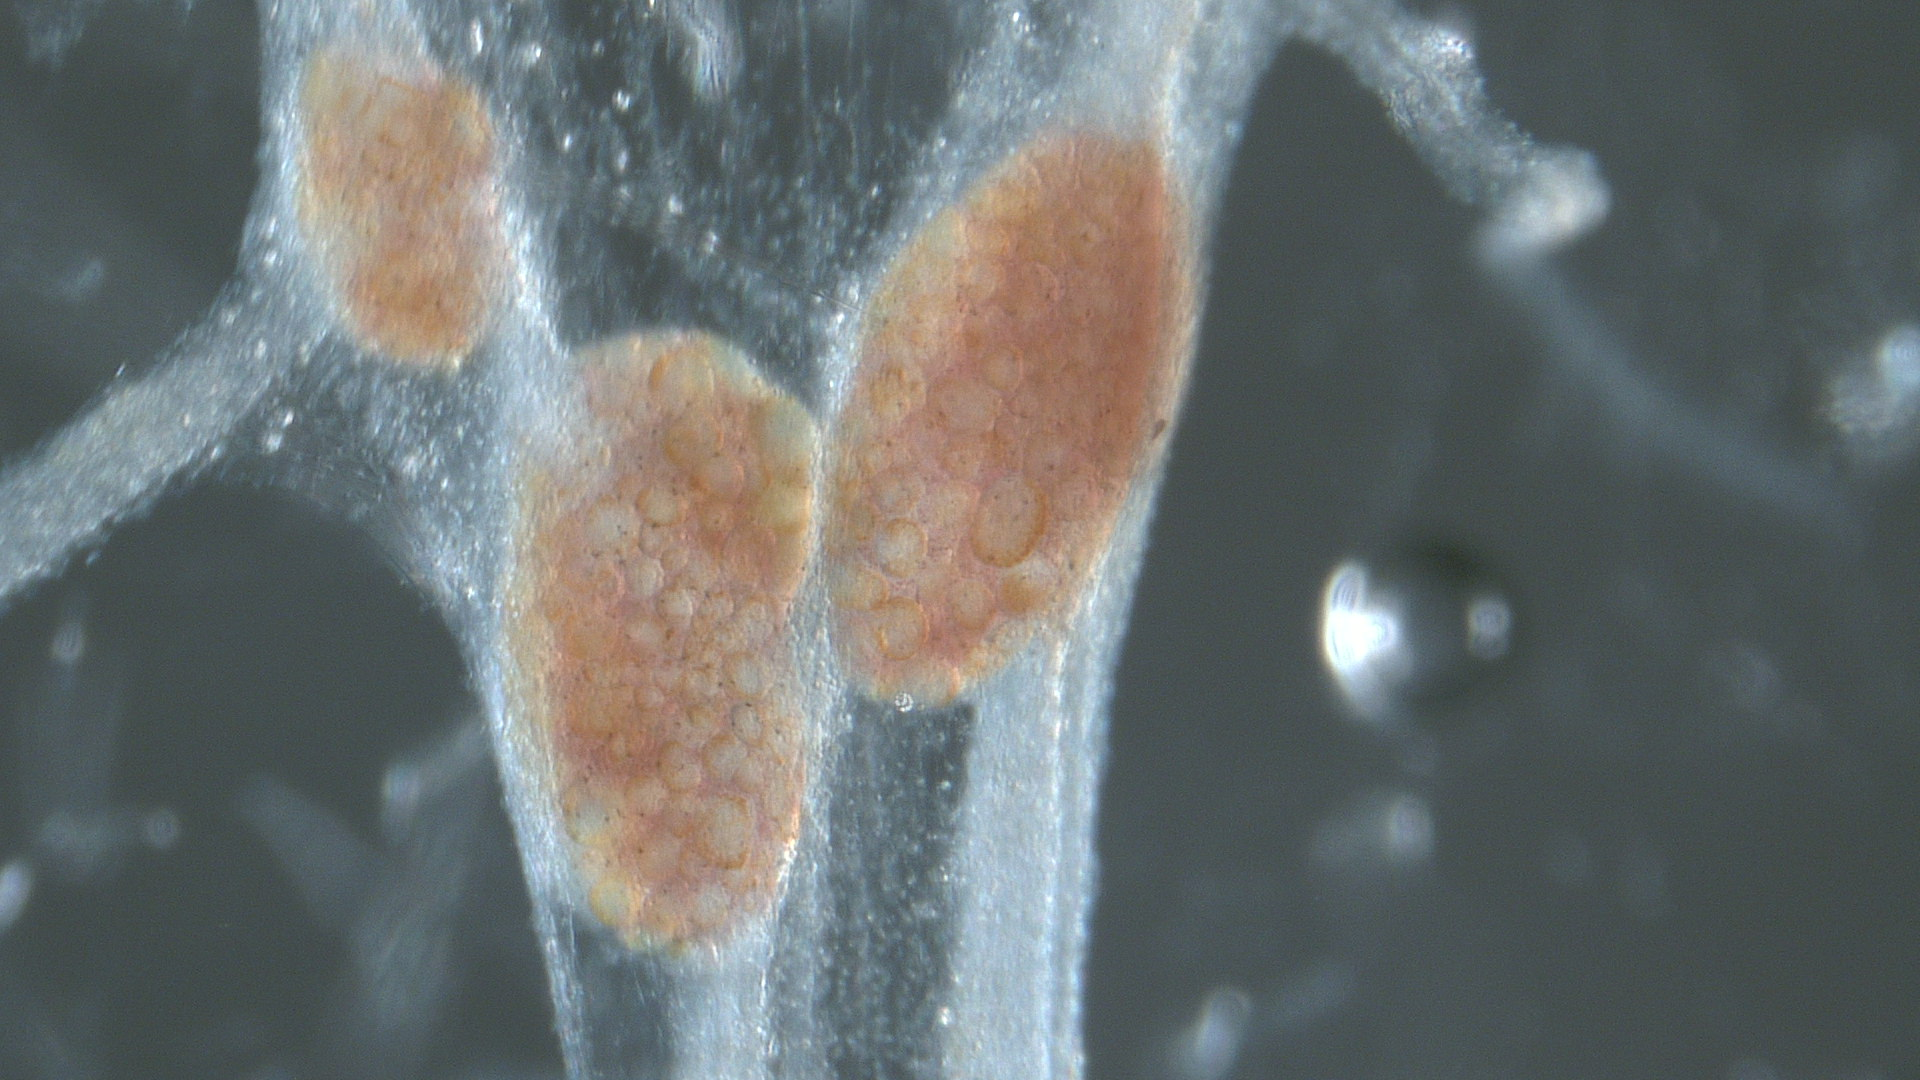
\includegraphics[width=0.9\linewidth]{img/methods/preparation/RPG.JPG}
    \endminipage
    \caption{Neural system of \textit{Lymnaea stagnalis}. a) Diagram of the neural system labeled for all ganglia. b) Top panel: photograph of the buccal ganglia. Bottom panel: photograph of the two parietal ganglia and visceral ganglion.}
    \label{fig:lymn neural sys}
\end{figure}

Neuronal recordings shown in this work are from the CPG in the buccal ganglia in chapter \ref{c-invariants}. In chapter \ref{c-laser} the recordings are from the right parietal ganglia (RPG), containing large neurons with tonic firing and a pair of electrically coupled giant cells in the RPG,  and from the visceral ganglia. These ganglia are illustrated in Fig. \ref{fig:lymn neural sys}b.

%%%% In contrast to other systems functionality where motoneurons are CPGs neurons \textcite{stomatogastric} ((page 5 review), in Lymnaea nervous system, CPGs and motoneurons are separated groups of neurons. 


\section{The feeding CPG of \textit{Lymnaea stagnalis}}
\subsubsection{Lymnaea feeding rhythm}

The feeding activity of the \textit{L. stagnalis}, concerning the buccal mass, is classified in three main steps: protraction, rasp and swallow, alternating with states of "rest". This sequence of buccal movements in the snail is generated by the motoneurons distributed in the ganglia. Each of these phases is associated to the activation of one interneuron from the CPG: N1M, N2v, N3t, and followed by the motoneurons associated to them. This is a complex distributed system where motoneurons do not exclusively follow the interneurons but are also implied in the feeding cycle activation \parencite{staras_patterngenerating_1998}. In this circuit, there are also some modulatory neurons involved such as the SO neuron (in the same buccal ganglia) or the CGC neuron (in the cerebral ganglia). Initial resting states, where the CPG as well as the motoneurons have no activity, may change due to a sensory input.

%\todo{revisar}% This input, received in the presence of food or during hunger, is handled in the cerebral ganglia generating activity and changing the SO tonic spiking during resting (which was inhibiting the CPG) to a bursting mode, meaning the start of the feeding cycle.

This CPG circuit can be studied in a dissected preparation, since snail neurons are active for a long time after the isolation of the system. Particularly, the CPG rhythm is maintained after its activation and it is generated autonomously by the neurons in the circuit. However, due to the slow dynamics of the system and the nature of the experimental setting, different ways to initiate the rhythm are also available for researchers. Previous literature in \textit{L. stagnalis} proposed several solutions to this problem. The first solution is stimulating the neurons responsible for the initiation of the feeding rhythm, such as the SO modulator neuron on the buccal ganglia, the CBC, or the CVs neurons, located on brain ganglia \parencite{benjamin_distributed_2012}. However, access to these neurons is not always easy and keeping them in constant stimulation might be necessary. Thus, another option for activation discussed in the literature is applying octopamine. Some neurons in the buccal ganglia are sensitive to octopamine and, as a result, this procedure activates the rhythm \parencite{vehovszky_octopaminecontaining_2004}. Alternatively, in a semi-intact preparation, sucrose can be applied to activate the rhythm \parencite{vavoulis_dynamic_2007,vehovszky_octopaminecontaining_2004,straub_endogenous_2002}. A similar approach performing a complete dissection consists in stimulating the Medium Lip Nerve (MLN). 
The recordings analyzed in chapter \ref{c-invariants} correspond to either spontaneous activity or to electrical stimulation in CV1a, SO neuron, or the Medium Lip Nerve (MLN).

\section{Electrophysiology in \textit{Lymnaea stagnalis}}

\label{subsec:preparation}
In this thesis, intracellular neuronal recordings have been carried out in the mollusk \textit{Lymnaea stagnalis}. Beyond the advantages of invertebrates discussed in section \ref{c-intro-invertebrates} -- its easily accessible neural system, and the size and resistance of its neurons to electrode impaling --, the great pond snail's neural system has been extensively described including the feeding CPG,  which is the model of study in chapter \ref{c-invariants} of this work. Also its slow dynamics are convenient when studying   the sequential evolution of the modulation in high temporal resolution, as in the case of the laser stimulation described in chapter \ref{c-laser}. 

The technique followed for neural activity acquisition was intracellular recordings with sharp electrodes filled with 3 M $KCl$. % Figure \ref{fig:membranepotential recording} there is a scheme of the potential measurement. Está en la intro.
 In this technique, a glass micropippete penetrates the cell to measure its electrical activity, with a minimal damage to the cell, and the evolution of the  membrane potential is then recorded using a DC amplifier (ELC-03M, NPI Electronic, Hauptstrasse, Tamm, Germany). Glass micropippetes were pulled using a Sutter Instruments puller (Model P-97) (see Figure \ref{fig:electrode}). Membrane potential recordings were acquired at 10 KHz using an A/D board (PCI-625 with a BNC-2090A DAQ device, National Instruments).

\begin{figure}[hbt!]
	\centering
	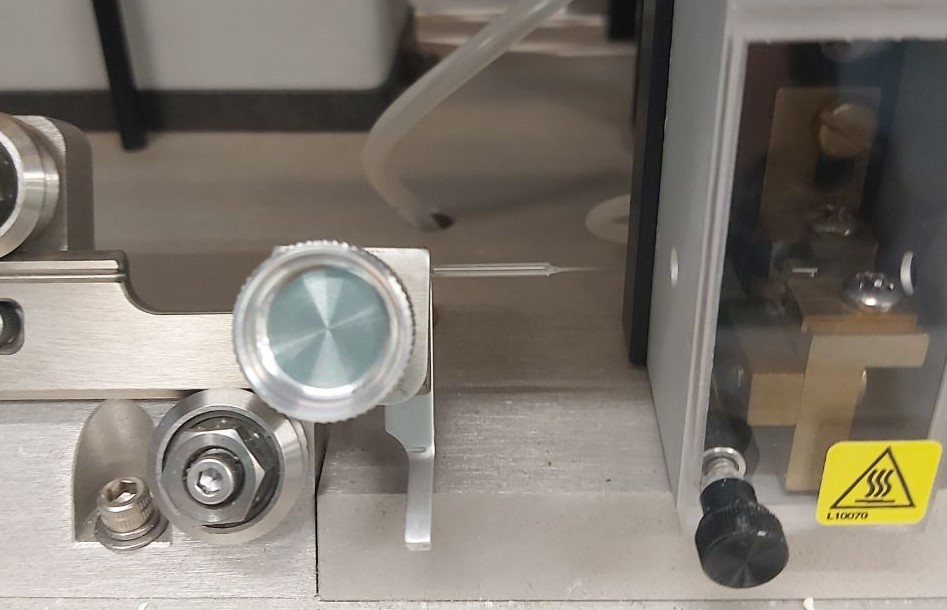
\includegraphics[width=0.6\linewidth]{img/methods/preparation/electrode4_zoom.jpg}
	\caption{Example of fabrication of a sharp micro-electrode glass in a pippete puller.}
	\label{fig:electrode}
\end{figure}
%todo: marcar con un circulo

To facilitate the access to the cell, the sheath above it was reduced using protease (Sigma XVII) over the ganglion for $\sim$1 min and then washed out with fresh saline (leaving the protease for longer time makes the impalement even more complicated due to the softness of the tissue). In order to record cell signals extra- and intracellularly, it is necessary to have full access to the neural system (see \cite{garrido-pena_tfm_2022} for more details). The preparation was immersed in a saline solution (in mM: 51.3 $NaCl$, 1.7 $KCl$, 1.5 $MgCl_2\cdot6H_2O$, 4.1 $CaCl_2\cdot2H_2O$, 5 $HEPES$, corrected to pH 7.8 with 4 $M$ $NaOH$). All procedures followed the European Commission and Universidad Autónoma de Madrid animal treatment guidelines.

The recordings analyzed in section \ref{sec:experimental sussex} were carried out using a equivalent procedure by Dr. Michael Crossley at the University of Sussex. 


\section{Conductance based models}
For the theoretical analyses in this work, we used simulations of conductance-based models. As discussed in section \ref{sec:computational neuroscience}, this kind of models are based on a specific combination of ionic channels with time-dependent conductance dynamics that provide a highly realistic description of the action potential generation. There are many different conductance-based models and formalisms depending on the specific combination of channels. Models used in this work, for both chapters \ref{c-invariants} and \ref{c-laser}, were designed for  neurons in \textit{Lymnaea stagnalis}, particularly for the neurons in the feeding CPG of the buccal ganglia --SO, N1M, N2v, N3t, \parencite{vavoulis_dynamic_2007}, for a neuron in the cerebral ganglia, CGC \parencite{vavoulis_balanced_2010}, and we also employed  the classical model by \textcite{hodgkin_quantitative_1952}. The feeding CPG model is a detailed description of the circuit with a combination of two-compartment neuron and  gradual synapse models, which allows sufficient flexibility in the circuit to induce variability from a current ramp stimulus --this will be discussed in detail in section \ref{c-invariants-model}. The second model --CGC model-- simulates a tonic firing and shoulder shaped spike waveforms, similar to the activity in some neurons in the right parietal ganglion characterized in chapter \ref{c-laser}.

\subsection{Feeding CPG model}
\label{sec:CPG model equations}
The \textcite{vavoulis_dynamic_2007} description of {\sl Lymnaea stagnalis} individual neurons considers a two-compartment model to represent the soma and the axon as  differentiated structures coupled by an axial resistance \parencite{vavoulis_dynamic_2007}. This separation of the soma and the axon is used to regulate the interaction between the fast and slow dynamics in the model. The slow dynamics are located at the soma, whereas the fast dynamics are included in the axon compartment. This distributed formalism is represented in Fig. \ref{fig:CPG diagram 2 compartments}a., where each circle represents either soma or axon, containing the different ionic currents for each one. The description of the voltage dynamics is provided for soma (Eq. \ref{eq:soma}) and axon (Eq. \ref{eq:axon}) compartments:

\begin{equation}
	\tau_m\frac{dV_S}{dt} = i_{inj} - i_{L,S} - i_X - i_{ec,S} - i_{syn} \\,
	\quad with \quad i_X = [i_{ACh},i_{NaL},i_T]
	\label{eq:soma}
\end{equation}

\begin{equation}
	\tau_m\frac{dV_A}{dt} = -i_{L,A} - i_{NaT} - i_K - i_{ec,A}
	\label{eq:axon}
\end{equation}

\noindent Here we follow the notation of \textcite{vavoulis_dynamic_2007} where $\tau_m$ represents the time constant of the membrane (in ms) given by the ratio of the membrane capacitance (in nF) and the leakage conductance (in $\mu$S). Below we will refer to the currents in capital leters as $I$, following the common notation. In equations \ref{eq:soma} and \ref{eq:axon}, $i$ variables (given in mV) are the product of the corresponding currents (in nA) times the passive input resistance given in M$\Omega$.
%, $i=I*R$, where  $R$ is given in M$\Omega$.

The soma compartment contains a slow current $I_X$ whose ionic nature depends on the specific CPG neuron described (see Fig.~\ref{fig:CPG diagram 2 compartments}a.). Thus, $I_X$  represents one channel, either $I_{ACh}$, $I_{NaL}$ or $I_{T}$, responsible of the specific slow dynamics associated with neurons N1M, N2v and N3t, respectively.  Along with the slow ionic channel and the leakage channel  $I_{L,S}$, the soma compartment also receives the synaptic current $I_{syn}$ and the injection current $I_{inj}$. All currents are explained in detail below.

On the other hand, fast channels are part of the axon compartment: a fast inactivating sodium current $I_{NaT}$ and a delayed rectifier potassium current $I_{K}$. These channels, along with the axon leakage channel  $I_{L,A}$ follow the definition in \textcite{hodgkin_quantitative_1952} model. The model cells as described above are not endogenously bursters so to achieve bursting activity, a distinct constant value of  \(i_{inj}\) is applied to the cells. 

The CPG topology scheme is shown in Fig. \ref{fig:CPG diagram 2 compartments}, where the connections between neurons are represented by dashed or solid lines, depending on whether the connection is slow or fast, respectively, and filled or empty circles at their end denoting the direction and the effect on the postsynaptic neuron: excitation (empty circles) or inhibition (filled circles).
Individual neurons following the previous description are connected by graded synapses, defined by equations \ref{eq:syn1}-\ref{eq:syn2} \parencite{vavoulis_dynamic_2007}. The differential point of a graded synapse is that it is dependent on voltage values and time, many synapses models used are just dependent on a trigger voltage value, that activates the synapse (see chapter \ref{c-intro-synapses} for details). This model of synapse allows dynamical adaptation of neurons in the circuit to maintain the rhythm despite even under induced variability. 

\begin{equation}
	i_{syn} = \sum_j \gamma_{syn,j} s_j (V_S - E_{syn,j})
	\label{eq:syn1}
\end{equation}

\begin{equation}
	\frac{ds_j}{dt} = \frac{r_{j}-s_j}{\tau_{syn,j}}
\end{equation}

\begin{equation}
	\frac{dr_j}{dt} = \frac{r_{\infty,j}-r_j}{\tau_{syn,j}}
\end{equation}

\begin{equation}
	r_{\infty,j}=\frac{1}{1+e^{(-40-V_{pre_{V_S}})/2.5}}
	\label{eq:syn2}
\end{equation}


\noindent where index $j$ runs over all presynaptic neurons and \(\gamma_{syn,j}, E_{syn,j},\tau_{syn},V_{pre_{V_S}}\) are the product of input resistance and maximal synaptic conductance, the synaptic reversal potential, the synaptic time constant and the presynaptic potential, respectively. 

The three inter-neurons described in this circuit have different waveform shapes, determined by their corresponding ionic channel and the axon connectivity, in Fig. \ref{fig:model simulation} there is an example of a simulation with all neurons in the circuit. First, N1M voltage characteristics are provided by an acetylcholine sensitive channel (\(i_{ACh} = 200 * p^3 * (V_S + 30)\)), which causes the gradual spiking frequency increase as well as the visible plateau, i.e., the slow wave is sustained before hyperpolarization. On the other hand, N2v has a slowly inactivating sodium channel (\(i_{NaL} = 2 * p^3 * q^3 * (V_S-55)\)), which causes the slow depolarization in this neuron. N2v neuron has a lower spiking frequency caused by the conductance value given for the axial $g_{ec}$ linking the two compartments, which is much lower in this cell. Finally, the N3t neuron has the particularity of a post inhibitory rebound, which generates an initial fast spiking followed by a decrease in the firing rate as the burst evolves. This latter property is caused by a low-threshold calcium channel (\( i_T = 3.27 * p^3 * q *(V_S-80)\)). SO neuron has no particular  \(I_X\) channel (in contrast to N1M, N2v, and N3t neurons) so its activity is the result of the combination of the common ionic channels in the axon and the soma.


\begin{figure}[htb!]
	\centering
	\begin{minipage}[t]{0.45\textwidth}
		\raggedright
		(a) \par
		\vspace{65pt}
		\centering
		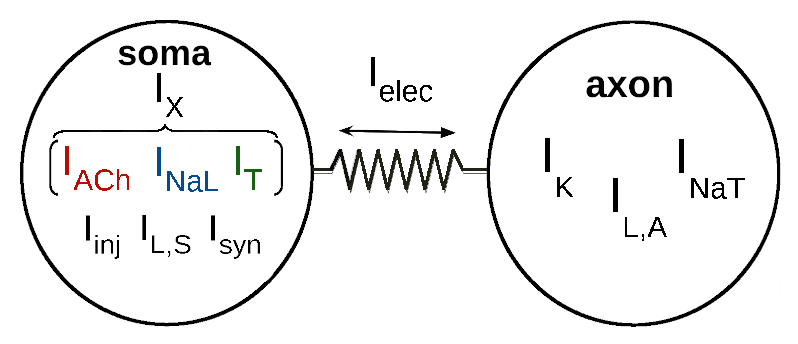
\includegraphics[width=\textwidth]{methods/invariants-model/figure1a.eps}
	\end{minipage}\hfill
	\begin{minipage}[t]{0.35\textwidth}
		\raggedright
		(b) \par
		\centering
		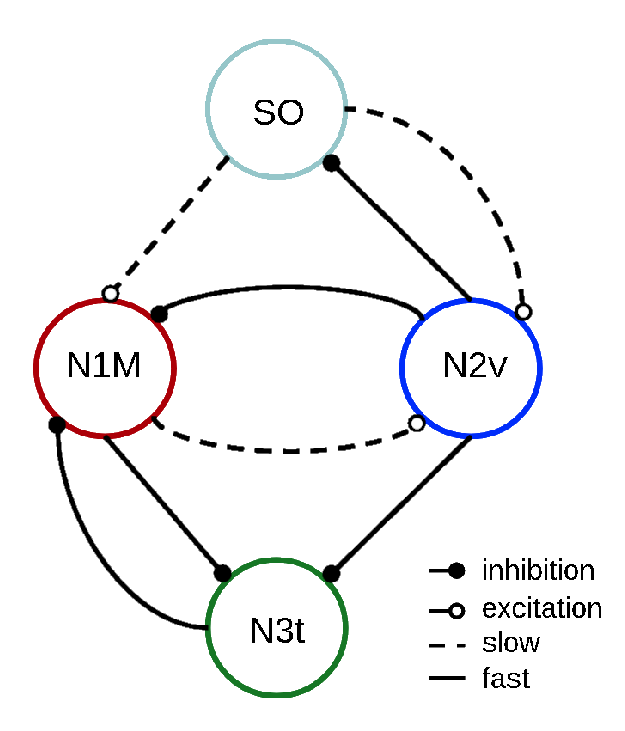
\includegraphics[width=\textwidth]{methods/invariants-model/figure1b.eps}
	\end{minipage}
	\caption{\textbf{Panel (a)}. Ionic channel distribution in the two-compartment description for the individual neurons in the \textcite{vavoulis_dynamic_2007} model used in this study. At the soma: $I_{ACh}$, acetylcholine ionic channel; $I_{NaL}$, slowly inactivating sodium
		ionic channel;$I_T$, low-threshold calcium current; $I_{inj}$, injected current; $I_{L,S}$, leakage current in the soma; $I_{syn}$, synaptic current. At the axon: $I_{NaT}$, fast inactivating sodium current; $I_K$, delayed rectifier potassium current; $I_{L,A}$, leakage current in the axon. The color for each $I_X$ current represents the CPG neuron that includes it at the soma,  N1M, N2v and N3t, respectively. \textbf{Panel (b)}. Connection scheme for the {\sl Lymnaea} feeding CPG circuit model. The colors indicating each neuron in the circuit match those in the representation of their corresponding somatic membrane potential traces in section \ref{sec:CPG model equations}. 
	}
	\label{fig:CPG diagram 2 compartments}
\end{figure}

\begin{figure}[htb!]
	\centering
	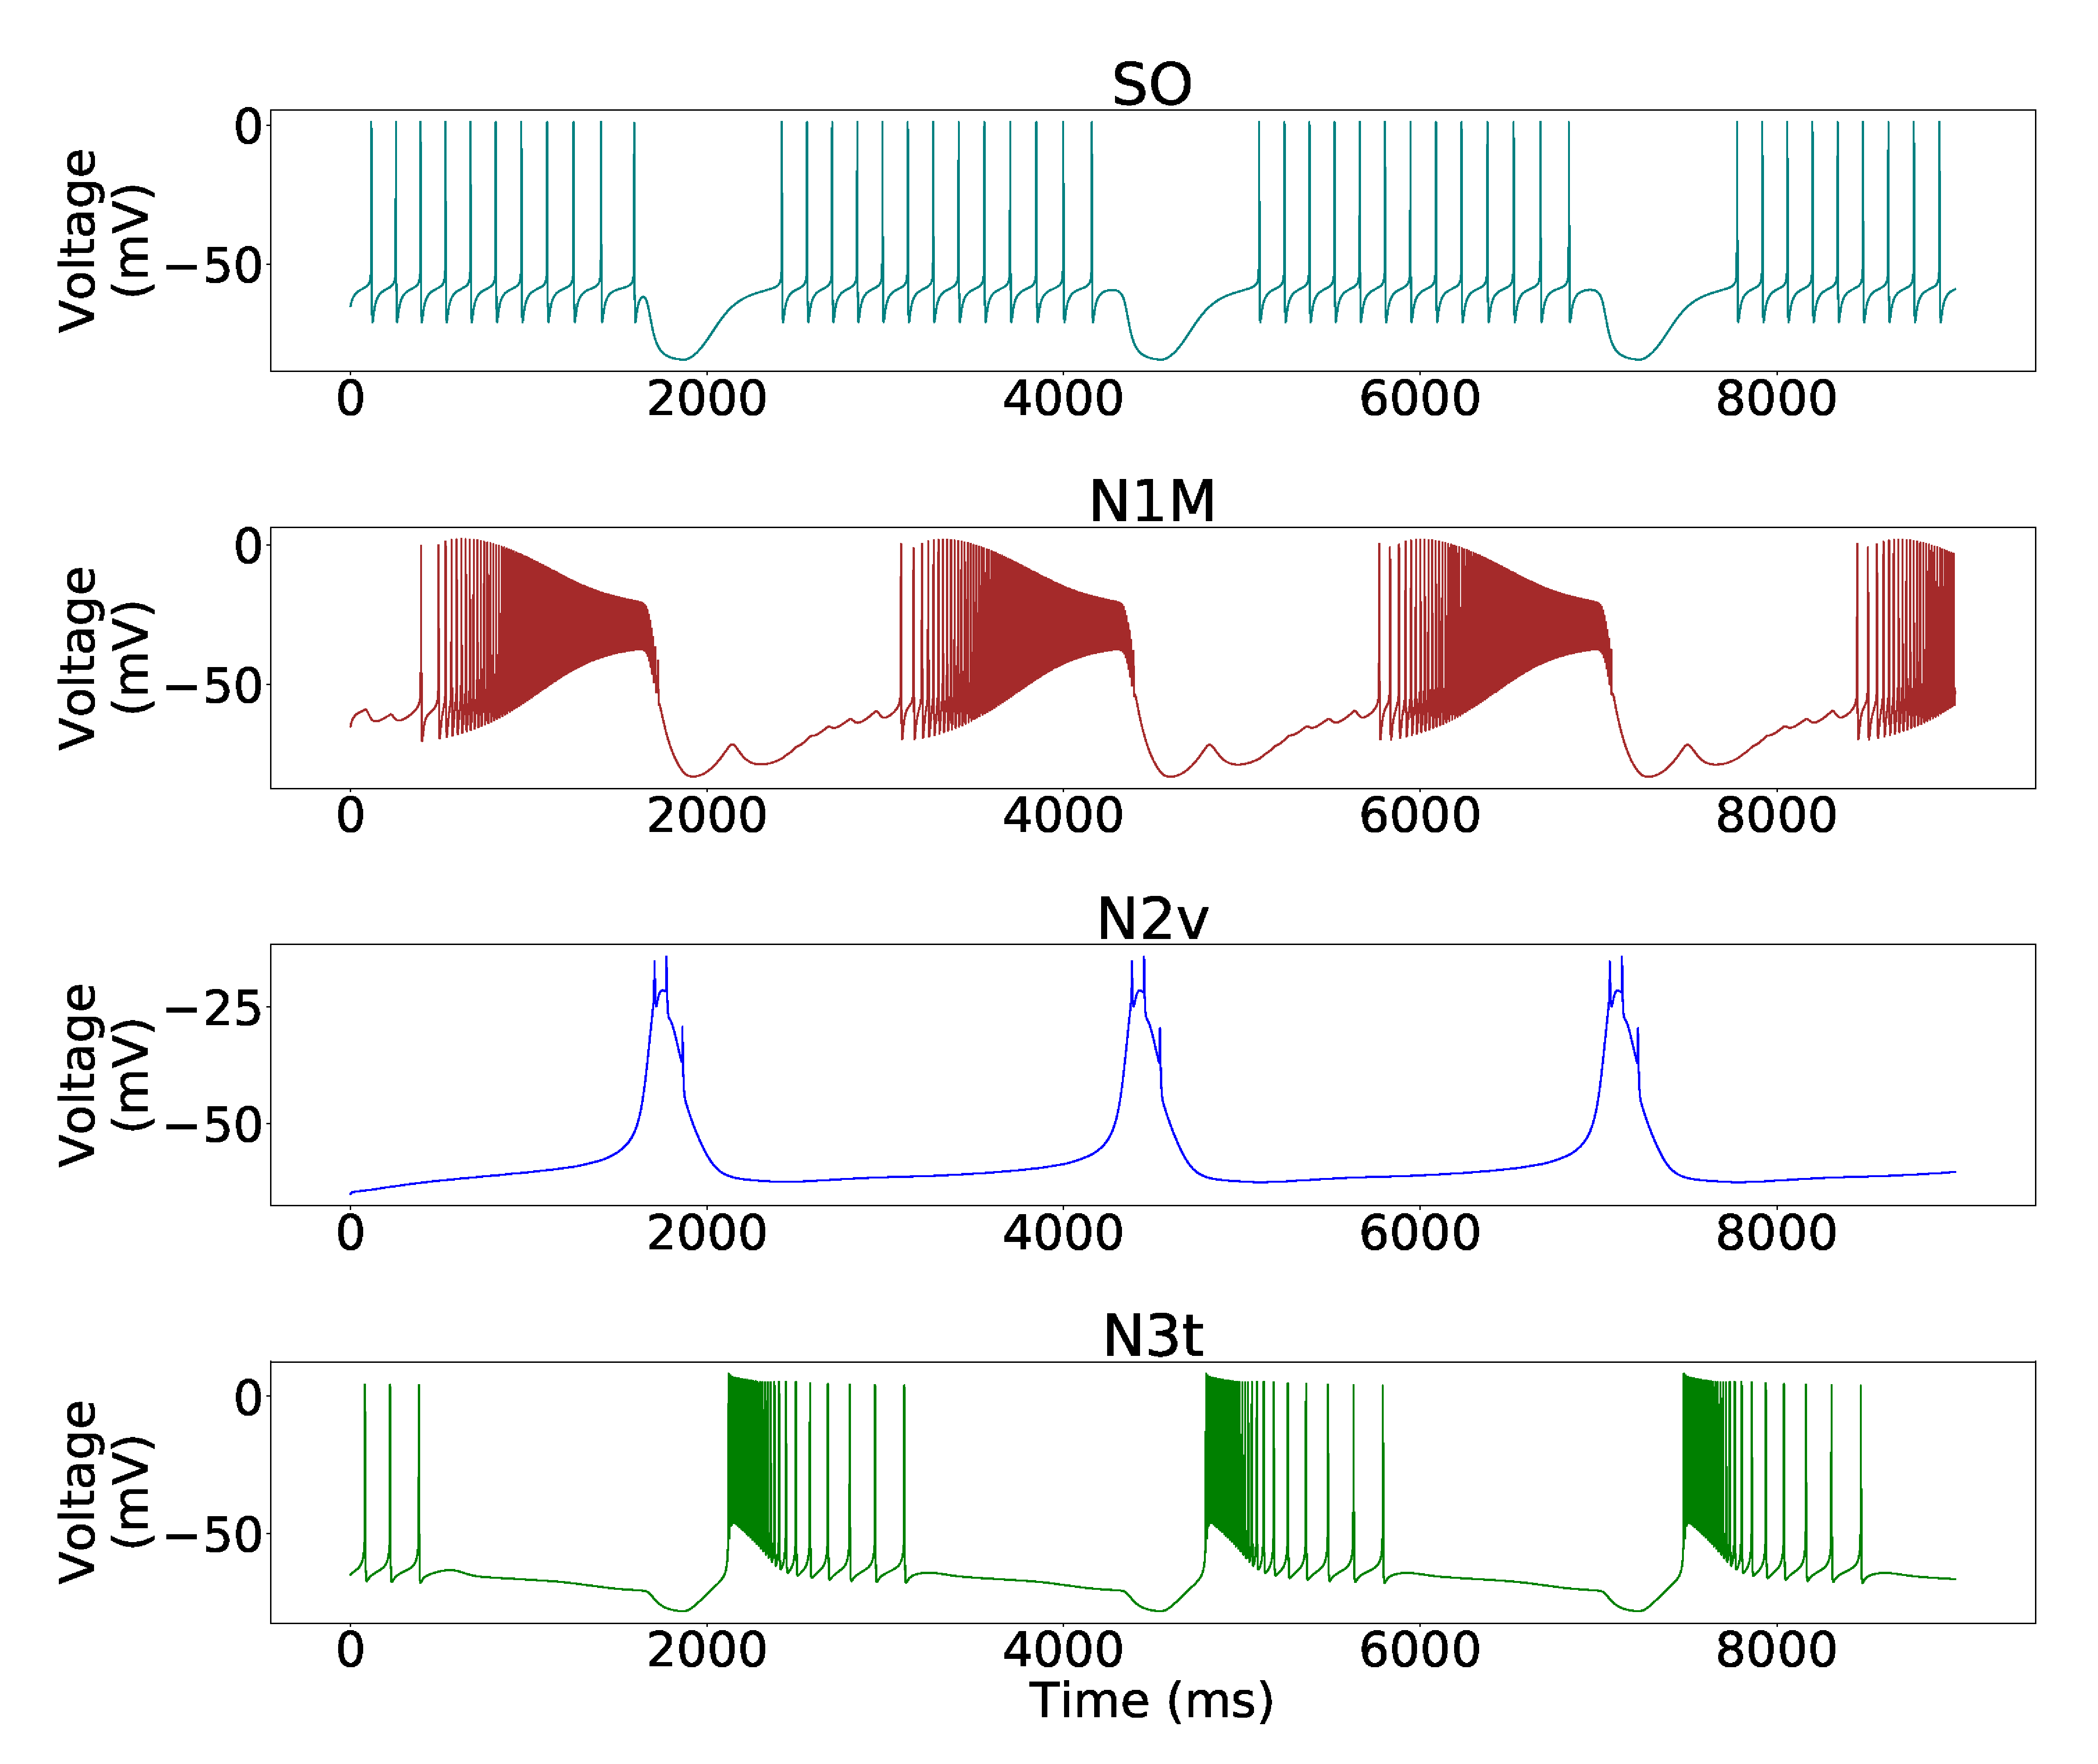
\includegraphics[width=0.7\linewidth]{methods/invariants-model/figure2.eps}
	\caption{Triphasic feeding rhythm as produced by the circuit CPG model described in Fig. \ref{fig:CPG diagram 2 compartments}. In this simulation, $i_{inj}$ values applied to each neuron are 8.5, 6, 2 and 0 mV, respectively.}
	\label{fig:model simulation}
\end{figure}



\subsection{CGC neuron model}
\label{subsec:cgc neuron model equations}
This model is described by six different ionic channels: Persistent and transient sodium currents ($I_{NaP}$, $I_{NaT}$), that primarily drive depolarization and action potential initiation; transient and delayed rectifier potassium currents ($I_A$, $I_D$), key for repolarization and contribute to the shoulder shape waveform in this neuron (specially $I_D$); and a low-voltage-activated and high-voltage-activated calcium currents ($I_{LVA}$, $I_{HVA}$), which are crucial for both immediate excitability and long-term plasticity. These channels are described by Eqs. \ref{eq:voltage} to \ref{eq:channels}. 

\begin{equation}
C_m\frac{dV}{dt} = I_{inj} - I_{NaT} - I_{NaP} - I_{A} - I_{D} - I_{LVA} - I_{HVA},
\label{eq:voltage}
\end{equation}

\begin{equation}
I_{NaT} = g_{NaT} m_{{\infty}}^3 h (V - E_{Na}),
\end{equation}
\begin{equation}
I_{NaP} = g_{NaP} r^3 (V - E_{Na}),
\end{equation}
\begin{equation}
I_{A} = g_{A} a^4 b (V - E_{K}),
\end{equation}
\begin{equation}
I_{D} = g_{D} n^4 (V - E_{K}),
% \label{eq:channels}
\end{equation}
\begin{equation}
I_{LVA} = g_{LVA} c_{{\infty}}^3 d_{{\infty}} (V - E_{Ca}),
\end{equation}
\begin{equation}
I_{HVA} = g_{HVA} e^3 f (V - E_{Ca}).
\label{eq:channels}
\end{equation}

Inactivation and activation dynamic variables $r,a,n,e$ and $h,b,f$ are defined by:
\begin{equation}
\frac{dx}{dt} = \frac{x_{\infty}-x}{\tau_x},
\end{equation}
where $x = h,r,a,b,n,e$ or $f$ and $x_{\infty}$ and $tau_x$ are defined by:

\begin{equation}
x_{\infty} = {(1+exp(\frac{V_H^x-V}{V_S^x}))}^{-1}
\end{equation}

See Supplementary Material in \textcite{vavoulis_balanced_2010} for more details. 

The implementation of this model is available at Neun library \href{https://github.com/GNB-UAM/neun}{github.com/GNB-UAM/neun} (VavoulisCGCModel).

\begin{figure}[htb!]
	\centering
	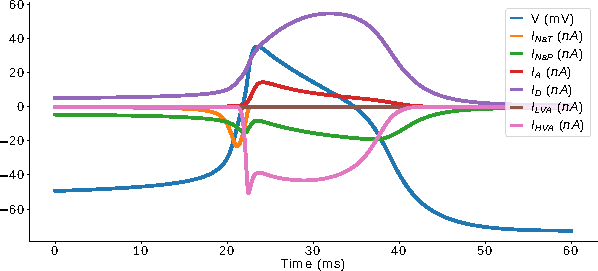
\includegraphics[width=\textwidth]{img/laser/cgc-model-simulation.pdf}
	\caption{Simulation of the CGC-model representing the voltage dynamics during an action potential and the corresponding ionic currents defined in the model ($I_{\textrm{NaP}}$,$I_{\textrm{NaT}}$, $I_{\textrm{A}}$, $I_{\textrm{D}}$, $I_{\textrm{LVA}}$,$I_{\textrm{HVA}}$). The units in the $y$-axis are specified in the legend.}
	\label{fig:model cgc currents}
\end{figure}


\subsubsection{Temperature dependence description in the model}
\label{sec:model equations temperature}
To simulate the temperature dependency in the neuronal activity, a $Q_{10}$ factor was incorporated to every dynamical equation in the model (i.e., conductances and activation gates). $Q_{10}$ represents temperature sensitivity in each channel and it was included as a new factor as shown in Eqs. \ref{Q10_conductance} and \ref{Q10_gates}, with $i=Na_T,Na_P,A,D,LVA,HVA$ for Eq. \ref{Q10_conductance} and $i=h,r,a,b,n,d,e,f$ for Eq. \ref{Q10_gates}. The capacitance was also defined as temperature dependent ($C_T$) with a linear relation to the difference of temperature: 

\begin{equation}g_i(T)=\bar{g}_i{Q^i_{10}}^{\frac{T-T_0}{10}},
\label{Q10_conductance}
\end{equation}
\begin{equation}\phi_i(T)=\bar{\phi}_i{Q^i_{10}}^{\frac{T-T_0}{10}},
\label{Q10_gates}\end{equation}
\begin{equation}C_T=c_0 + c_0 \gamma(T-T_0).\end{equation}


where $\bar{g}_i$, $\bar{\phi}_i$, $c_0$ are the original values used in the model and $\gamma = 0.05$.

 
\section{Neural data analysis}
%Detectar eventos --> secuencia
% Eventos promediados ocultan información --> secuencialidad ciclo a ciclo
%Métricas

To analyze the recordings of intracellular signals and the outputs of the models' simulations, we relied on the detection of single events, mainly spikes. Thus, we either defined time-intervals for the CPG rhythm or analyze each single spike based on waveform metrics as described in chapter \ref{c-laser}. The detection of these time references (e.g., the duration of a spike or the first and last spike in a burst) allowed us to study the sequentiality of neural dynamics at different time-scales. In the cycle-by-cyclle analysis, we focused on each event and cycle, avoiding the averaging of the results, since we consider this hinders information in the analysis of the sequential activity. 

For the study of the time-intervals variability and the presence of sequential dynamical invariants, the spikes of the recording were detected by a voltage threshold, i.e., all peaks over a voltage value were considered action potential peaks and spikes in the model simulation of the bursting activity were detected using the change in the derivative along with a similar voltage threshold condition. Then, bursts were identified from the temporal structure of the spikes, and intervals were characterized by the timing of the first and last spike in each burst. In some recordings these temporal references were adjusted to the needs of the data available, this will be specified in the corresponding section \ref{sec:experimental sussex}.

All intervals defined in section \ref{subsec:intervals} were defined by the events in the \textit{beginning} and \textit{end} of the burst, the time-intervals described were characterized as follows:

%For the boxplots, the Python library matplotlib.pyplot used each cycle-by-cycle interval duration. Linear regression from sklearn Python library was used to quantify the relation of the sequence intervals to the instantaneous period of each cycle. 

\begin{lstlisting}
	#########  SINGLE INTERVALS
	# on = 0; off = 1
	
	# off1 - on1 of the burst duration
	def get_burst_duration(data):
		return np.array([b - a for a, b in zip(data[:, 0], data[:, 1])])
	
	# on2 - off1 of one burst and the next one, respectively
	def get_burst_interval(data):
		return np.array([a - b for a, b in zip(data[1:, 0], data[:, 1])])
		
	# on2 - on1 of one burst and the next one, respectively
	def get_burst_period(data):
		return np.array([a - b for a, b in zip(data[1:, 0], data[:, 0])])
		
	#########  PAIRED INTERVALS
	def get_intervals(d1,d2):
		if d1.size == 0 or d2.size == 0:
			return [],[]
			
		d1d2_interval = np.array([b-a for a,b in zip(d1[:,0],d2[:,0])])
		d1d2_delay = np.array([b-a for a,b in zip(d1[:,1],d2[:,0])])
		d2d1_interval = np.array([a-b for a,b in zip(d1[1:,0],d2[:-1,0])])
		d2d1_delay = np.array([a-b for a,b in zip(d1[1:,0],d2[:-1,1])])
	
		return [d1d2_interval,d1d2_delay],[d2d1_interval,d2d1_delay]
\end{lstlisting}

On the other hand, to analyze the data obtained from recordings and model simulations of the tonic firing activity for the CW-NIR laser effect analysis, we based on the spike waveform. To detect the spike times, it was usually enough with a voltage threshold to detect the events in the sequence --regarding the stereotyped spike waveform. To analyze the waveform after the detection of the events, each time event in the voltage signal was segmented by considering $N$ milliseconds before and after the event, thus defining segments that capture the shape of the waveform. The characterization of that waveform was carried by defining four metrics: duration, amplitude, and depolarization and repolarization slopes. The characterization of these metrics was implemented as follows:

\begin{lstlisting}
	# Description: 
	# 	Recives spike voltage values and return the time values to get the duration time 
	#	measured at the mid point of the spike waveform 
	# Parameters:
	# 	spike: voltage values
	# 	dt: time rate
	# 	thres_val: voltage value where to measure the duration. By the fault mid point. 
	#	v_scale: scale of the voltage, assumes mV
	# Return:
	#	time points at middle point of the spike waveform. 
def get_spike_duration(spike,dt, thres_val=0.5, v_scale=1): 
	spike = spike[~np.isnan(spike)]
	
	peaks, properties = find_peaks(spike, prominence=1*v_scale, width=20)
	
	if len(peaks)>1: # in case spike has several peaks, gets mid one.
		mid_peak = np.isclose(len(spike)//2, peaks, atol=10)
		peaks = peaks[mid_peak]
	results_half = peak_widths(spike, peaks, rel_height=thres_val)
	
	
	# get the two time points corresponding to the waveform at midpoint
	try: 
		duration_vals = np.array([results_half[2][0], results_half[3][0]])
		th = results_half[1]
	except Exception as e:
		duration_vals = np.array([])
		th = 0
	
	if duration_vals.size == 0: #Safety comprobation
		return (0,0),th
	else:
		return (duration_vals[0]*dt,duration_vals[-1]*dt),th
	
# Description:
# 	Calls get_spike_duration function and returns a single time value of the duration
# 	with the difference of the two points returned by the previous function.
def get_spike_duration_value(waveform, dt, plot=False, v_scale=1):
	dur_refs,th = get_spike_duration(waveform, dt, plot=plot, v_scale=v_scale)
	duration = dur_refs[1]-dur_refs[0]
	return duration

# Description: 
# 	Recives spike values and return the amplitude value measured as the distance between
#	maximum and minimum voltage value.
# Parameters:
# 	spike voltage values
# 	dt time rate
# Return:
#	amplitude
def get_spike_amplitude(spike,dt, v_scale=1):
	spike = spike[~np.isnan(spike)] 
	mx_value = np.max(spike) #maximum V value (spike)
	mn_value = np.min(spike) #minimum V value (spike)

	return mx_value-mn_value

# Description: 
# 	Recives spike values and return the increasing and decreasing slope values at the 
#	two points matching a threshold in "the middle" of the spike maximum and minimum voltage value.
# Parameters:
# 	spike voltage values
# 	dt time rate
# 	n_points: number of points around position to calculate slope
#   slope_position: where to calculate slope: defalult value, mid of spike.
# Return:
#	depolarization slope, repolarization slope 

def get_slope(spike,dt,n_points=10, slope_position=0.5, plot=False, v_scale=1):
	spike = spike[~np.isnan(spike)] 
	mid_ps,th = get_spike_duration(spike,dt,thres_val=slope_position, v_scale=v_scale)
	indx1 = int(mid_ps[0]/dt) #From ms to point ref
	indx2 = int(mid_ps[1]/dt) #From ms to point ref
	
	scale = int(0.1/dt)
	n_points *= scale
	
	n_ms = n_points*dt
	
	slope1 = (spike[indx1+n_points]-spike[indx1-n_points])/(n_ms*2) 
	slope2 = (spike[indx2+n_points]-spike[indx2-n_points])/(n_ms*2)

	return (slope1,slope2)
\end{lstlisting}

Finally, the model were implemented in $C++$ taking advantage of its computational speed. Most analyses were performed in Python3, since it is a frequently used tool and libraries such as Pandas are very effective for data analysis. Some spike detection analysie of the intracellular recordings of the CPG were performed in the visual tool DataView \parencite{heitler_dataview_2007}. Scripts used in this work are available at \href{https://github.com/agarpe/neural-dynamics-utils}{github.com/agarpe/neural-dynamics-utils} and all conductance-based models are included in Neun \href{https://github.com/GNB-UAM/Neun}{github.com/GNB-UAM/Neun}


\section{CW-NIR laser setup}
The experimental results presented here were obtained using a continuous-wave (CW) NIR diode laser in single TEM00 operation and 830nm wavelength output (Integrated Optics 0830L-13A-NI-PT-NF). 
\begin{wrapfigure}{l}{0.4\textwidth}
    \centering
	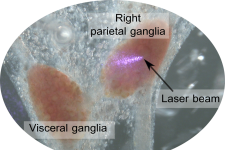
\includegraphics{img/laser/laser-beam.png}
	\caption{Illustration of the laser beam focused on a neuron in the right parietal ganglia.}
	\label{fig:laser beam}
\end{wrapfigure} 
Figure \ref{fig:laser setup} shows the experimental setup. The diode laser output was coupled to a single-mode optical fiber to efficiently guide the laser beam to the sample. To adapt the divergence of the laser beam to the fiber optic output, an aspherical lenses-collimator (Thorlabs, F280FC-850) was installed. An achromatic doublet with focal length f=50mm was used to focus the laser beam on the sample (Thorlabs AC127-050-B-ML). The experiments were performed with a laser output power of $\sim$ 90 mW and a power density over the sample of 146 W/cm². The grazing incidence of the laser beam on the sample created a quasi-elliptical spot, with a minor axis of approximately 34{\textmu}m, as shown in Fig. \ref{fig:laser beam}.

\begin{figure}[htb!]
	\centering
	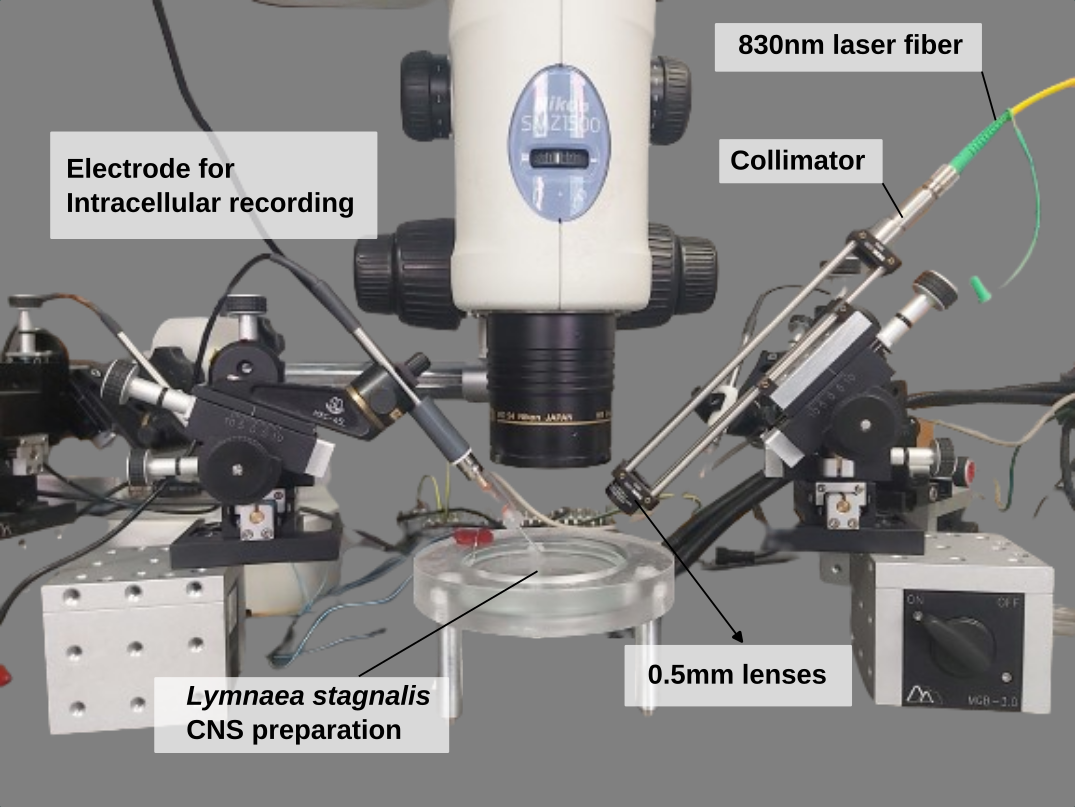
\includegraphics[width=0.65\textwidth]{img/methods/laser-setup_labels.png}
	\caption{Image of the NIR-laser stimulation setup. On the left, there is the micromanipulator with the electrode and the glass micropipette for the intracellular recording. In the center of the image under the microscope lens, there is the preparation of the CNS of \textit{Lymnaea stagnalis}. On the right side, the laser fiber is attached to the collimator and at the end of the holder there is a lens to focus the laser beam. This is also attached to a micromanipulator for a precise focusing.}
	\label{fig:laser setup}
\end{figure}

The laser was attached to a micro-manipulator (Siskiyou MX160), allowing micrometer precision of the beam placement over the neuron and optimization of the beam focus. The focusing was performed using a binocular microscope (Nikon SMZ-1500) coupled to a CCD camera (XCAM1080PHA, ToupTek Photonics, Zhejiang, China).
